\documentclass[10pt,a4paper]{article}
\usepackage[utf8]{inputenc}
\usepackage{polski}
\usepackage{amsmath}
\usepackage{amsfonts}
\usepackage{amssymb}
\usepackage{graphicx}
\usepackage{verbatim}
\usepackage{minted}
\usepackage{amsmath}
\usepackage{algorithm}
\usepackage[noend]{algpseudocode}
\usepackage{csvsimple}
\usepackage{caption}
\usepackage{subcaption}
\makeatletter
\def\BState{\State\hskip-\ALG@thistlm}
\makeatother

\author{Onaszkiewicz Przemysław, Gadawski Łukasz}
\title{Rozwiązanie zadania komiwojażera przy pomocy algorytmu genetycznego. \\ 1) Wersja sekwencyjna i zrównoleglona \\ (pamięć wspólna).}

\begin{document}
\maketitle

\section{Cel zadania}
Celem pierwszego etapu projektu jest implementacja wersji sekwencyjnej algorytmu genetycznego działającego na pojedynczym procesorze do rozwiązywania problemu komiwojażera. A także zastosowanie dyrektyw \textit{OpenMP} w celu dokonania zrównoleglenia wykonania algorytmu na wielu procesorach z pamięcią wspólną.

\section{Problem komiwojażera}
Problem zdefiniowany jest następująco: mając listę miast oraz odległości między nimi, znajdź najkrótszą, dozwoloną drogę (początkiem oraz końcem drogi jest ten sam wierzchołek), zawierającą każde miasto dokładnie raz. Przy czym można zacząć od dowolnego miasta oraz kolejność miast jest dowolna. Inaczej problem polega na znalezieniu minimalnego cyklu Hamiltona w pełnym grafie ważonym. Problem należy do zbioru problemów NP-trudnych.

\section{Algorytm genetyczny}
W 1975 roku przez Johna Hollanda został wynaleziony algorytm genetyczny, którego zadaniem było działanie analogiczne do procesu ewolucji na ziemi. Pseudokod prostego algorytmu genetycznego (ang. \textit{Simple Genetic Algorithm}) został przedstawiony w pseudokodzie \textit{Algotithm 1}.

\begin{algorithm}
\caption{Simple Genetic Algorithm}\label{euclid}
\begin{algorithmic}[1]
\Procedure{Simple Genetic Algorithm}{}

\State $\textit{t} \gets \text{0}$
\State $\text{initilize } P^{t}$
\State $\text{evaluate } P^{t}$

\BState \emph{while (\textbf{not stop\_condition})}:
\State $O^{t} \gets \text{reproduce } P^{t}$
\State $\text{crossover } O^{t}$
\State $\text{mutate } O^{t}$
\State $\text{evaluate } O^{t}$
\State $P^{t + 1} \gets O^{t}$
\State $t \gets t + 1$

\EndProcedure
\end{algorithmic}
\end{algorithm}
%\begin{minted}{bash}
%procedure "Simple Genetic Algorithm"
%begin 
%	t := 0
%	initilize P^{t}
%	evaluate P^{t}
%	while (not stop_condition)
%	begin
%		O^{t} = reproduce P^{t}
%		crossover O^{t}
%		mutate O^{t}
%		evaluate O^{t}
%		P^{t + 1} := O^{t}
%		t := t + 1
%	end
%end
%\end{minted}

Sterowanie algorytmem genetycznym odbywa się poprzez warunek stopu, którym może być satysfakcjonująca wartość funkcji celu lub ilość generacji. Typowy algorytm genetyczny rozpoczyna się inicjacją populacji wstępnej. W przypadku problemu komiwojażera \textbf{populacją} będzie lista osobników, natomiast każdy \textbf{osobnik} będzie konkretną listą miast, czyli jednym ze stanów z całej przestrzeni stanów. W przypadku problemu komiwojażera przestrzenią stanów jest zbiór wszystkich możliwych kombinacji dróg pomiędzy miastami. Następnie dokonywana jest ocena wartości każdego osobnika w populacji. W naszym przypadku będzie to obliczenie drogi każdego z zainicjowanych stanów. Kolejno następuje \textit{reprodukcja} populacji, która zostanie opisana dokładniej w kolejnym punkcie. Następnie wykonywane są operacje krzyżowania oraz mutacji, czyli "urozmaicanie" aktualnej populacji, a w dalszej części wytypowanie populacji, która będzie stanowiła listę najlepszych osobników do reprodukcji w kolejnej generacji.

\subsection{Reprodukcja}
Reprodukacja polega na wytypowaniu osobników do populacji potomnych, ale tak aby preferować osobniki lepiej przystosowane, czyli posiadające lepszą wartość funkcji przystosowania. Ocena jakości osobników dokonywana jest na podstawie funkcji przystosowania. W przypadku problemu komiwojażera mniejsza droga jest lepszym rezultatem, a zatem dąży się do minimalizacji drogi, którą reprezentuje każdy osobnik. Podczas reprodukcji następuje losowy wybór osobników do populacji potomnej, ale prawdopodobieństwo wylosowania każdego z nich nie jest jednakowe. W przypadku osobników lepiej przystosowanych występuje większe prawdopodobieństwo. Wartość prawdopodobieństwa obliczana jest zgodnie z następującym wzorem: 

$p_i = \frac{len\_sum - len_i}{\sum_{i}^{I} (len\_sum - x_i)}$, gdzie \\ 
$len\_sum$ - suma długości wszystkich osobników w populacji, \\
$len_i$ - długość i-tego osobnika, dla którego jest liczone prawdopodobieństwo,

Następnie mając prawdopodobieństwa osobników w populacji następuje obliczenie dystrybuanty prawdopodobieństwa. Podczas losowania osobników następuje losowanie liczby z przedziału $(0.00, 1.00)$, a następnie wybranie osobnika, który odpowiada danej wartości dystrybuanty. Taki dobór nazywany jest selekcją ruletkową (ang. \textit{round-wheel selection}).

\subsection{Mutacja}
Operacja mutacji wykonywana jest z określoną wartością prawdopodobieństwa, która jest parametrem algorytmu. Zgodnie z prawdopodobieństwem podejmowana jest decyzja o zmutowania konkretnego osobnika. Proces polega na losowej zamianie pozycji dwóch miast w początkowej liście miast. Dzięki temu zostaje wprowadzone całkowicie losowe zróżnicowanie dwóch osobników. Przeważnie wartość tego parametru ustawiona jest na niską wartość, tak aby wprowadzać różnorodność w każdym pokoleniu, ale aby również nie zakłócać polepszania wartości funkcji dostosowania w pokoleniu.

\subsection{Krzyżowanie}
Operacja krzyżowania również ma na celu wprowadzenie różnorodności w osobnikach w kolejnych pokoleniach. Jest wykonywana z określoną wartością prawdopodobieństwa, która jest parametrem algorytmu. Wszystkie osobniki w populacji są dobierane w pary. Następnie dla każdej z pary zgodnie z parametrem jest podejmowana decyzja o dokonaniu operacji krzyżowania. W dalszej kolejności losowane zostają indeksy krzyżowania. Elementy osobników pomiędzy tymi indeksami zostają zamienione między osobnikami. A elementy osobników znajdujące się poza indeksami zostają przepisane począwszy od wylosowanego indeksu. Geny(miasta), które już znajdują się w osobniku są pomijane. T gwarantuje że osobnik po krzużowaniu będzie osobnikiem prawidłowym (każge miasto będzie odwiedzone tylko raz).

\section{Implementacja}

\subsection{Tworzenie mapy miast}
W naszej implementacji mapa została odwzorowana jako obiekt posiadający wielkość, zbiór miast oraz strukturę danych \textit{mapa} gdzie kluczem jest para miasto-miasto oraz odległość między taką na mapie.

\subsubsection{Wczytanie z pliku}
Mapę odległości między miastami można odczytać z pliku tekstowego o strukturze przedstawionej poniżej. W pierwszej linii pliku znajdują się wierzchołki grafu oddzielone tabulatorami. W kolejnych liniach znajdują się krawędzie grafu(po jednej krawędzi na linię) w postacie wierzchołek - wierzchołek - wartość. Separatorem w pliku jest tabulator. Przykład pliku przedstawiono poniżej.

\begin{minted}{bash}
0	1	2	3
0	1	100
0	2	10
0	3	10
1	2	20
1	3	70
2	3	50
\end{minted}{bash}
\subsubsection{Losowa generacja mapy}

Możliwa jest losowa generacja mapy poprzez wywołanie metody :
\begin{minted}{bash}
shared_ptr<Map> Map::ConstructMapOfSize(int mapSize,
		int lowestPossibleDistance = 0, int highestPossibleDistance = 200)
\end{minted}
Podana metoda konstruuje mapę miast o zadanej wielkości, która jest grafem pełnym. Krawędzie grafu które są odległościami między miastami mają losowe wartości pomiędzy wartościami zadanymi w parametrach  \textit{lowestPossibleDistance i highestPossibleDistance}. 

\subsection{Konfiguracja programu}
Konfiguracja programu jest możliwa przy pomocy pliku \textit{app.properties}. Umożliwia on zdefiniowanie następujących parametrów:
\begin{itemize}
\item[--] \textbf{population\_size} - wielkość populacji w każdej iteracji algorytmu,
\item[--] \textbf{propability\_of\_crossover} - prawdopodobieństwo krzyżowania,
\item[--] \textbf{propability\_of\_mutation} - prawdopodobieństwo mutacji,
\item[--] \textbf{generation\_number} - liczba pokoleń, czyli iteracji algorytmu, w przypadku naszej implementacji jest to warunek stopu.
\end{itemize}

Przykładowa zawartość pliku konfiguracyjnego została zamieszczona poniżej.
\begin{minted}{bash}
population_size=5
propability_of_crossover=0.20
propability_of_mutation=0.01
generation_number=3
\end{minted}
\section{Testy}
Przeprowadzono testy z działania programu. Dzielą się one na dwie części. Pierwszą z nich jest Sprawdzenie poprawności algorytmu na niewielkich grafach. Kolejną jest przetestowanie efektywności zrównoleglenia algorytmu.
\subsection{Testy poprawności}
Jako dane wejściowe sprawdzające poprawność działania algorytmu wykorzystano dwa, małe, tendencyjnie stworzone grafy, w których można z łatwością dokonać weryfikacji działania algorytmu.Schematy podanych grafów przedstawiono poniżej.

\begin{figure}[H]
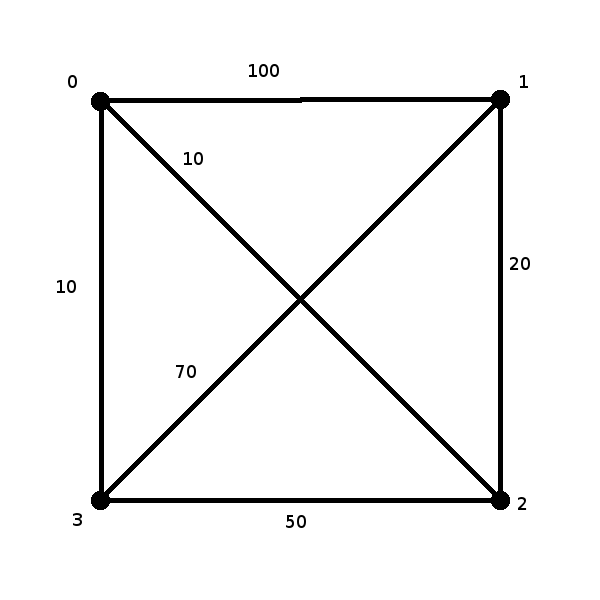
\includegraphics[scale=0.5]{mapa4.png}
\centering
\caption{\label{graph4}Graf wejściowy zawierający 4 wierzchołki}
\end{figure}
Po przetworzeniu pliku wejściowego zawierającego graf \ref{graph4} Algorytm wyznaczył najkrótszą ścieżkę o wartości 110. Należy pamiętać że ostatnim odcinkiem pokonywanym przez kuriera jest droga z ostatniego odwiedzonego miasta do miasta z którego wyruszył. W tym przypadku jest to krawędź pomiędzy wierzchołkami 1 i 3 o wartości 70. Najważniejsze fragmenty pliku wejściowego zostały przedstawione poniżej. 

\begin{minted}{bash}
POPULATION SIZE: 30

map size: 4
nodes:0 1 2 3 
m[first city: 0 sec city: 1] = 100
m[first city: 0 sec city: 2] = 10
m[first city: 0 sec city: 3] = 10
m[first city: 1 sec city: 2] = 20
m[first city: 1 sec city: 3] = 70
m[first city: 2 sec city: 3] = 50


Initial population initialization time: 7154 microseconds

START reproduce

START reproduce
0 'st generation production time: 22464 microseconds

START reproduce
1 'st generation production time: 14053 microseconds

START reproduce
2 'st generation production time: 9021 microseconds

START reproduce
3 'st generation production time: 362 microseconds

START reproduce
4 'st generation production time: 339 microseconds

START reproduce
5 'st generation production time: 357 microseconds

whole loop time 46596

 END: 3->0->2->1

PAth LEN: 110
\end{minted}{bash}

\begin{figure}[H]
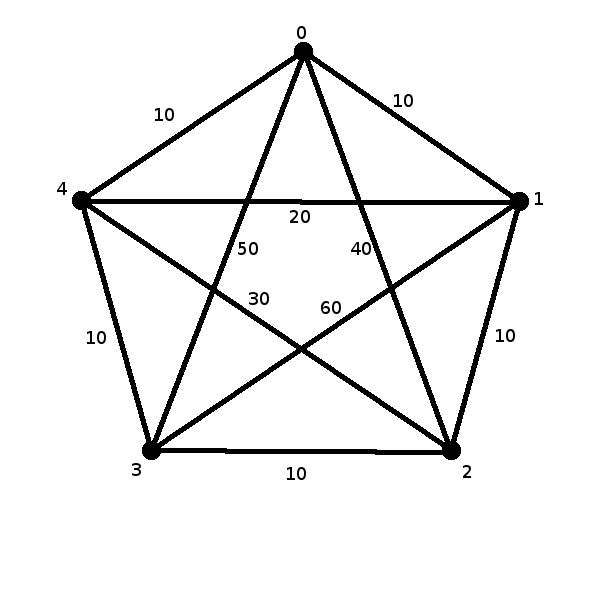
\includegraphics[scale=0.5]{mapa5.png}
\centering
\caption{\label{graph5}Graf wejściowy zawierający 5 wierzchołków}
\end{figure}

Po przetworzeniu pliku z grafem wejściowym przedstawionego na rysunku \ref{graph5} program wyznaczył ścieżkę o wartości 50. Najważniejsze fragmenty pliku wejściowego zostały przedstawione poniżej.

\begin{minted}{bash}
map size: 5
nodes:0 1 2 3 4 
m[first city: 0 sec city: 1] = 10
m[first city: 0 sec city: 2] = 40
m[first city: 0 sec city: 3] = 50
m[first city: 0 sec city: 4] = 10
m[first city: 1 sec city: 2] = 10
m[first city: 1 sec city: 3] = 60
m[first city: 1 sec city: 4] = 20
m[first city: 2 sec city: 3] = 10
m[first city: 2 sec city: 4] = 30
m[first city: 3 sec city: 4] = 10


Initial population initialization time: 8892 microseconds

START reproduce

START reproduce
0 'st generation production time: 14998 microseconds

START reproduce
1 'st generation production time: 14012 microseconds

START reproduce 
2 'st generation production time: 14433 microseconds

START reproduce
3 'st generation production time: 11731 microseconds

START reproduce 
4 'st generation production time: 12254 microseconds

START reproduce
5 'st generation production time: 18946 microseconds

whole loop time 86374

END: 4->0->1->2->3

PAth LEN: 50
\end{minted}{bash}

\subsection{Testy efektywności zrównoleglenia}
Kolejnym etapem testów było przetestowanie efektywności zrównoleglenia kodu. Wykorzystanie poszczególnych rdzeni procesora zostało przedstawione na rysunkach poniżej. Jeden z nich przedstawia wykonanie szeregowe programu, drugi zaś wykonanie zrównoleglone.


\begin{figure}[H]
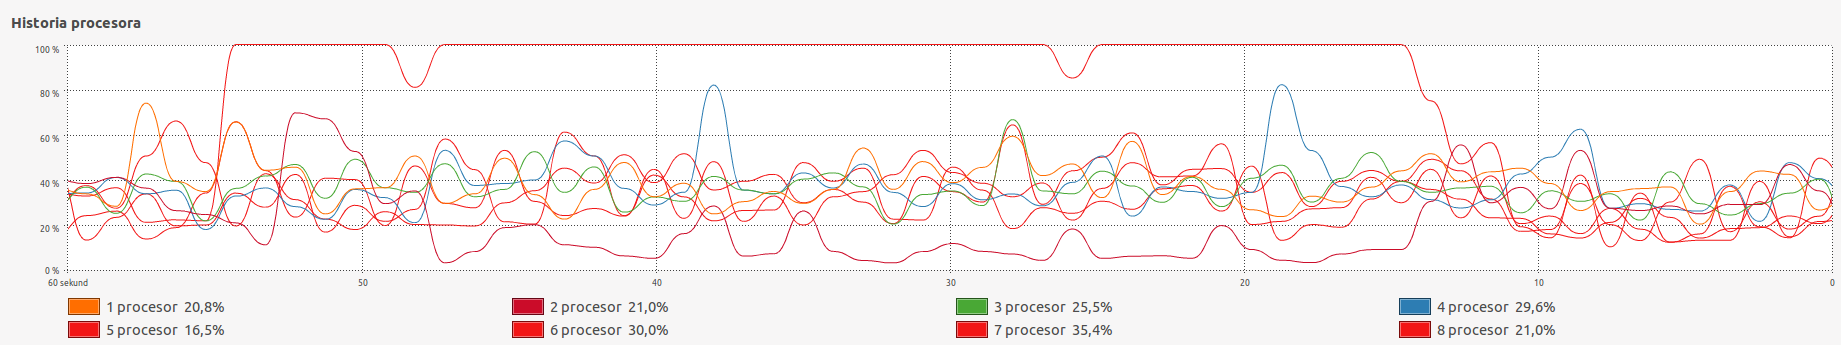
\includegraphics[scale=0.18]{zrzutSequence.png}
\centering
\caption{\label{diagramSequence}Diagram przedstawiający zużycie wątków przy wykonaniu sekwencyjnym}
\end{figure}

\begin{figure}[H]
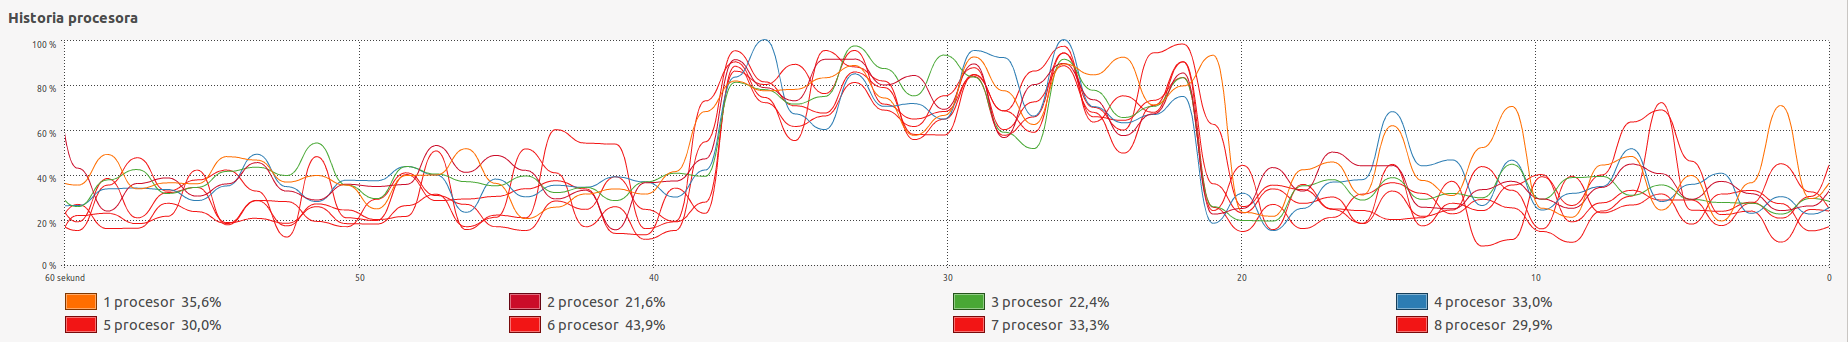
\includegraphics[scale=0.18]{zrzutParallel.png}
\centering
\caption{\label{diagramParallel}Diagram przedstawiający zużycie wątków przy wykonaniu zrównoleglonym}
\end{figure}

\subsection{Wyniki testów\label{sec:wt}}
W poniższej tabeli przedstawiono wyniki testów. dla kilku wykonań z różną ilością wątków, różną ilością miast i wielkością populacji.


%\csvstyle{myTableStyle}{tabular=|,
%table head=\hline \raggedright{ LICZBA  WĄTKÓW} & LICZBA  MIAST & WIELKOŚĆ  POPULACJI & LICZBA POKOLEŃ & CZAS WYKON. & RYS\\
%\hline\hline
%}

%\csvreader[myTableStyle]{tabela.csv}
%{\thecsvrow \csvcoli & \csvcolii}%
\begin{table}[H]
\begin{tabular}{|p{2cm}|p{2cm}|p{2.2cm}|p{2cm}|p{2.5cm}|p{2cm}|}
\hline
LICZBA  WĄTKÓW & LICZBA  MIAST & WIELKOŚĆ  POPULACJI & LICZBA POKOLEŃ & CZAS WYKON. & RYS\\
\hline
1 & 100 & 50 & 10 &	1685526 & \ref{fig:11-1}\\\hline
2 &	100 & 50 & 10 &	1411701 & \ref{fig:11-2}\\\hline
4 & 100 & 50 & 10 &	1373483 & \ref{fig:11-4}\\\hline
8 &	100 & 50 & 10 &	1360702	& \ref{fig:11-8}\\\hline
\\\hline
1&	500&	50&	10&	73504041&	\ref{fig:31-1}\\\hline
2&	500&	50&	10&	41945947&	\ref{fig:31-2}\\\hline
4&	500&	50&	10&	27070634&	\ref{fig:31-4}\\\hline
8&	500&	50&	10&	25775216&	\ref{fig:31-8}\\\hline
\\\hline			
1&	100&	100&	10&	4020926&	\ref{fig:32-1}\\\hline
2&	100&	100&	10&	3303909&	\ref{fig:32-2}\\\hline
4&	100&	100&	10&	3131004&	\ref{fig:32-4}\\\hline
8&	100&	100&	10&	3179381&	\ref{fig:32-8}\\\hline
\\\hline					
1&	500&	100&	10&	145557350&	\ref{fig:33-1}\\\hline
2&	500&	100&	10&	85992390&	\ref{fig:33-2}\\\hline
4&	500&	100&	10&	71970985&	\ref{fig:33-4}\\\hline
8&	500&	100&	10&	54755121&	\ref{fig:33-8}\\\hline
\hline

\end{tabular}
\caption{Tabela przedstawiająca wyniki czasowe w zależności od liczby miast, rozmiaru populacji i ilości wątków}
\end{table}

\begin{figure}[H]
    \centering
    \begin{subfigure}[b]{0.4\textwidth}
        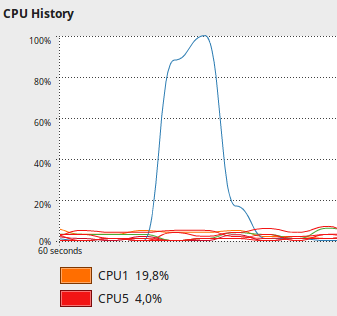
\includegraphics[width=\textwidth]{11-1.png}
        \caption{Jeden wątek}
        \label{fig:11-1}
    \end{subfigure}
    \begin{subfigure}[b]{0.4\textwidth}
        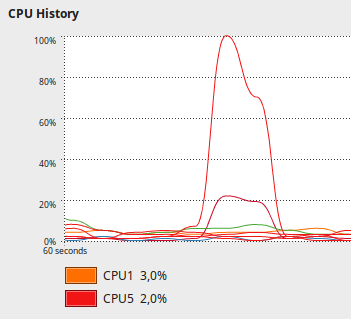
\includegraphics[width=\textwidth]{11-2.png}
        \caption{Dwa wątki}
        \label{fig:11-2}
    \end{subfigure}
    
    \begin{subfigure}[b]{0.4\textwidth}
        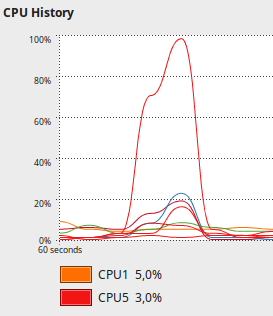
\includegraphics[width=\textwidth]{11-4.png}
        \caption{Cztery wątki}
        \label{fig:11-4}
    \end{subfigure}
    \begin{subfigure}[b]{0.4\textwidth}
            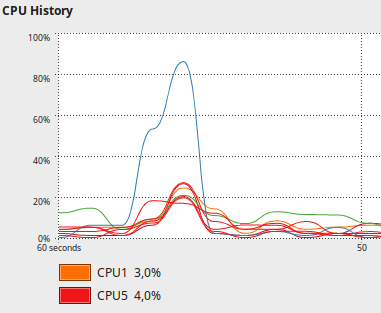
\includegraphics[width=\textwidth]{11-8.png}
            \caption{Osiem wątków}
            \label{fig:11-8}
    \end{subfigure}
    \caption{Fragmenty schematu ilustrującego zużycie rdzeni procesora przy użyciu (\ref{fig:11-1}) 1 wątku, (\ref{fig:11-2}) 2 wątków, (\ref{fig:11-4}) 4 wątków, (\ref{fig:11-8}) 8 wątków przy 50 miastach i wielkości populacji równej 100(pierwsze 4 wiersze tabeli)}\label{fig:11}. 
\end{figure}

\begin{figure}[H]
    \centering
    \begin{subfigure}[b]{\textwidth}
        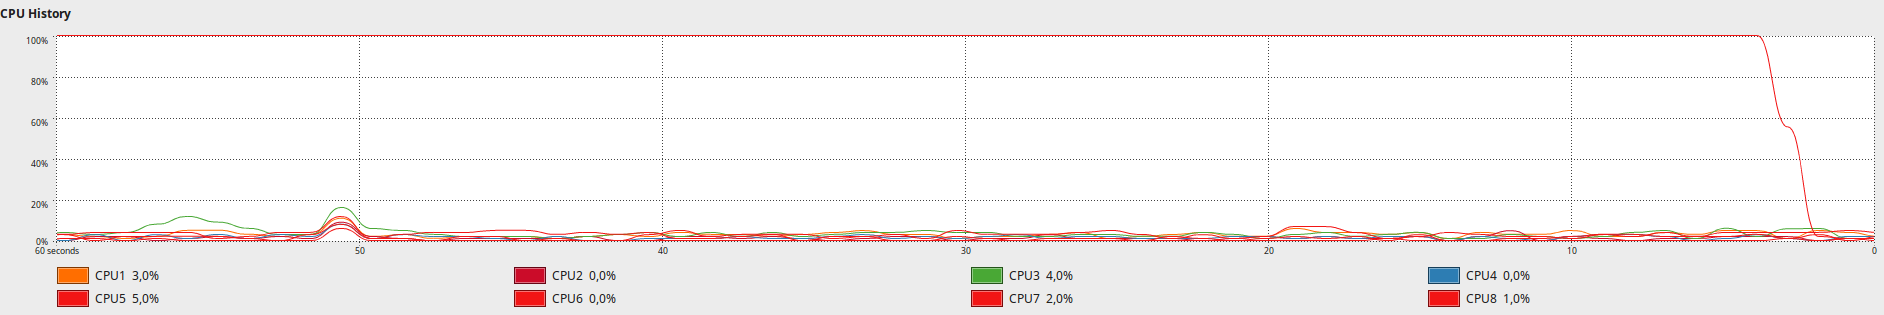
\includegraphics[width=\textwidth]{31-1.png}
        \caption{Jeden wątek}
        \label{fig:31-1}
    \end{subfigure}
    
    \begin{subfigure}[b]{\textwidth}
        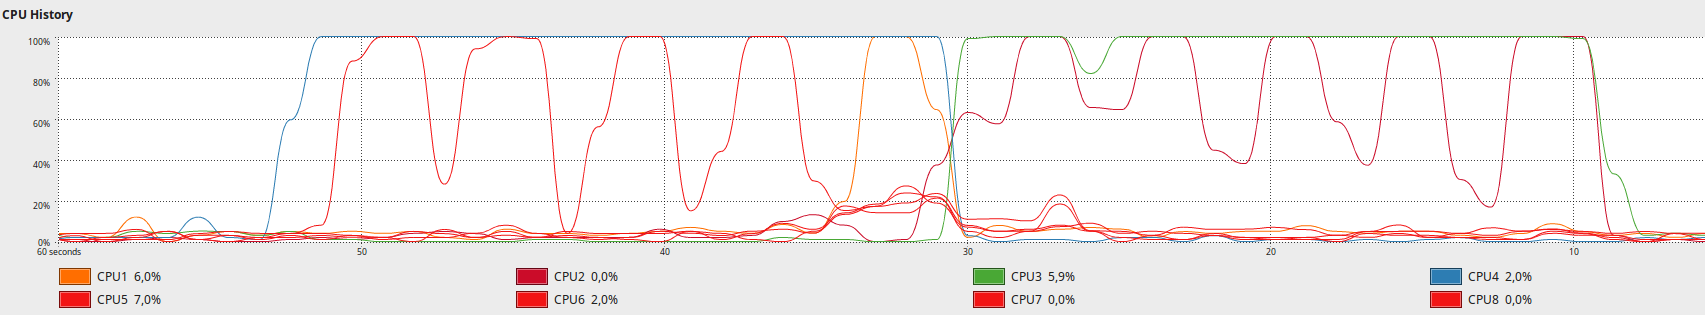
\includegraphics[width=\textwidth]{31-2.png}
        \caption{Dwa wątki}
        \label{fig:31-2}
    \end{subfigure}
    
    \begin{subfigure}[b]{\textwidth}
        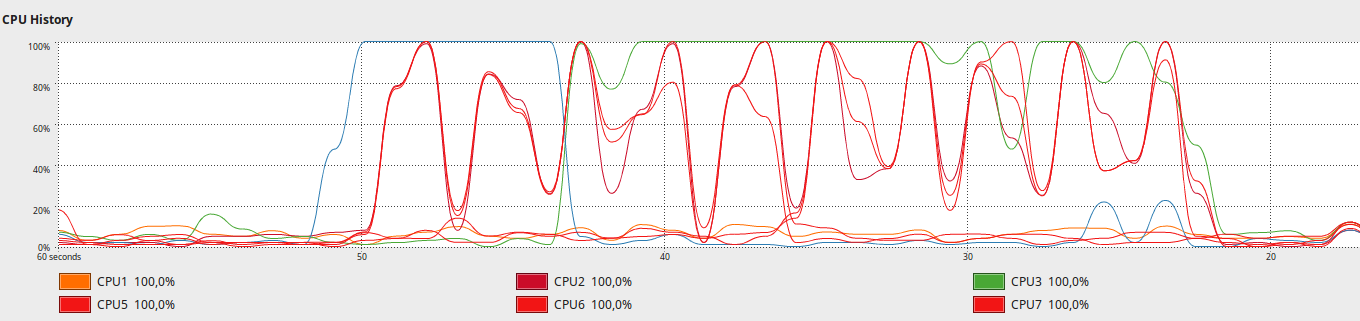
\includegraphics[width=\textwidth]{31-4.png}
        \caption{Cztery wątki}
        \label{fig:31-4}
    \end{subfigure}
    
    \begin{subfigure}[b]{\textwidth}
            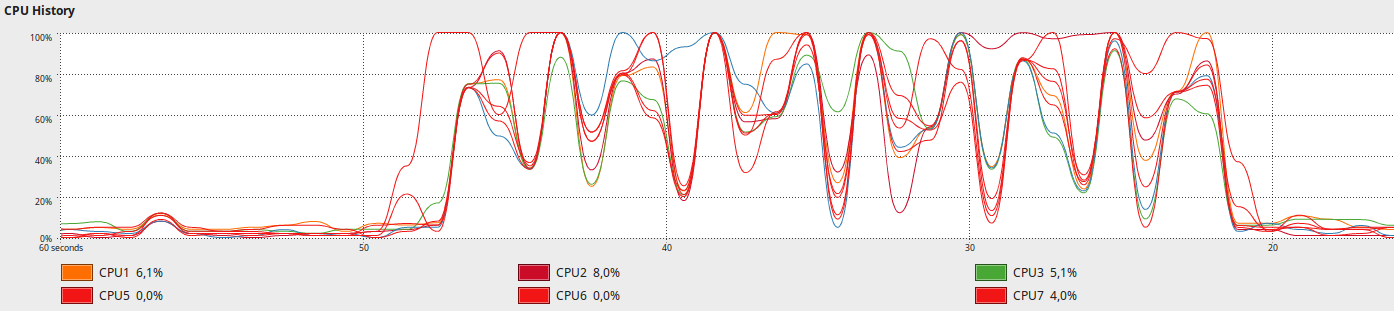
\includegraphics[width=\textwidth]{31-8.png}
            \caption{Osiem wątków}
            \label{fig:31-8}
    \end{subfigure}
    \caption{Fragmenty schematu ilustrującego zużycie rdzeni procesora przy użyciu (\ref{fig:31-1}) 1 wątku, (\ref{fig:31-2}) 2 wątków, (\ref{fig:31-4}) 4 wątków, (\ref{fig:31-8}) 8 wątków przy 500 miastach i wielkości populacji równej 50(drugie 4 wiersze tabeli)}\label{fig:31}. 
\end{figure}

\begin{figure}[H]
    \centering
    \begin{subfigure}[b]{\textwidth}
        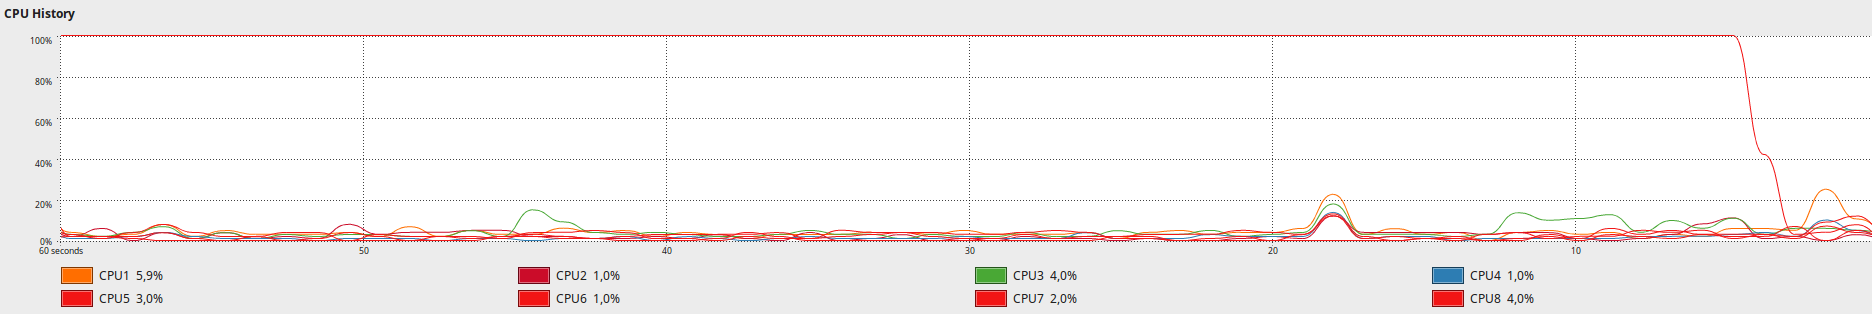
\includegraphics[width=\textwidth]{32-1.png}
        \caption{Jeden wątek}
        \label{fig:32-1}
    \end{subfigure}
    
    \begin{subfigure}[b]{\textwidth}
        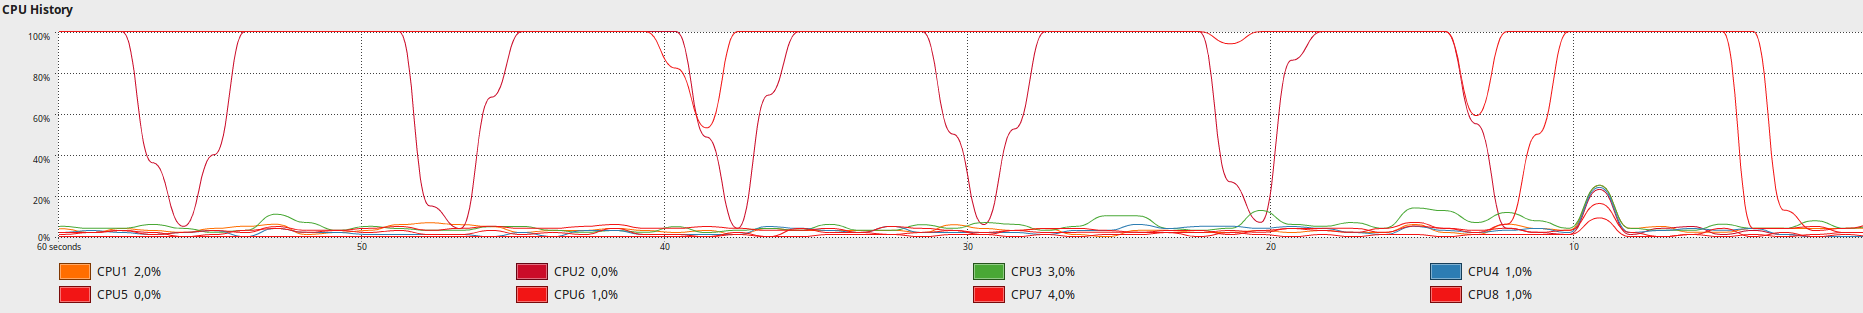
\includegraphics[width=\textwidth]{32-2.png}
        \caption{Dwa wątki}
        \label{fig:32-2}
    \end{subfigure}
    
    \begin{subfigure}[b]{\textwidth}
        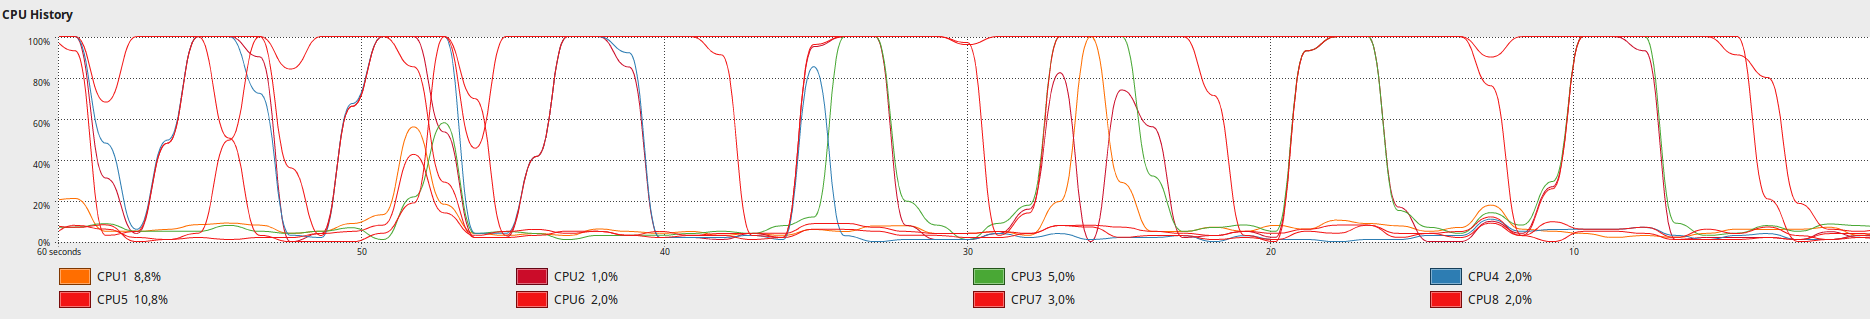
\includegraphics[width=\textwidth]{32-4.png}
        \caption{Cztery wątki}
        \label{fig:32-4}
    \end{subfigure}
    
    \begin{subfigure}[b]{\textwidth}
            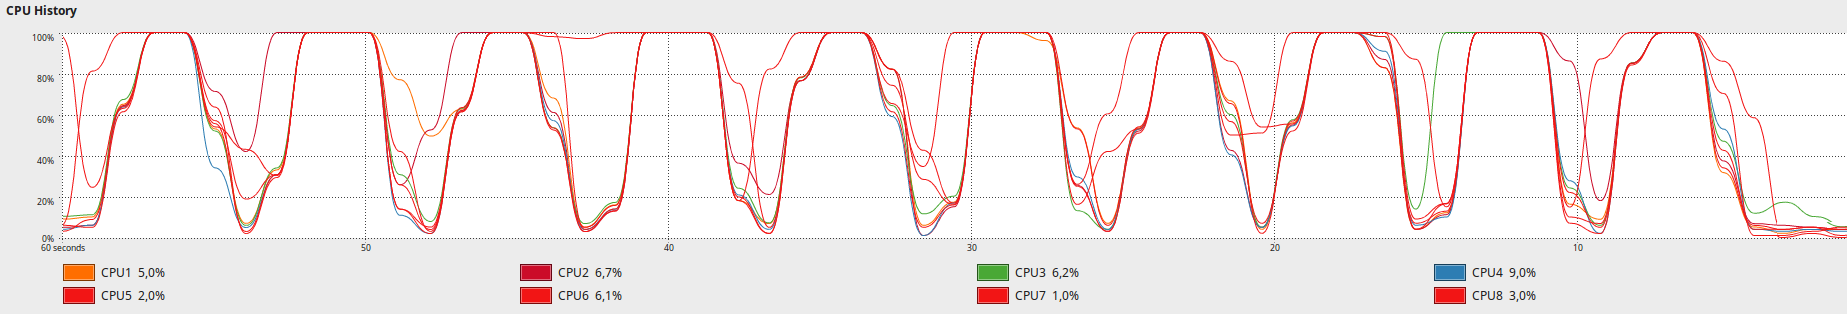
\includegraphics[width=\textwidth]{32-8.png}
            \caption{Osiem wątków}
            \label{fig:32-8}
    \end{subfigure}
    \caption{Fragmenty schematu ilustrującego zużycie rdzeni procesora przy użyciu (\ref{fig:32-1}) 1 wątku, (\ref{fig:32-2}) 2 wątków, (\ref{fig:32-4}) 4 wątków, (\ref{fig:32-8}) 8 wątków przy 100 miastach i wielkości populacji równej 100(trzecie 4 wiersze tabeli)}\label{fig:32}. 
\end{figure}

\begin{figure}[H]
    \centering
    \begin{subfigure}[b]{0.4\textwidth}
        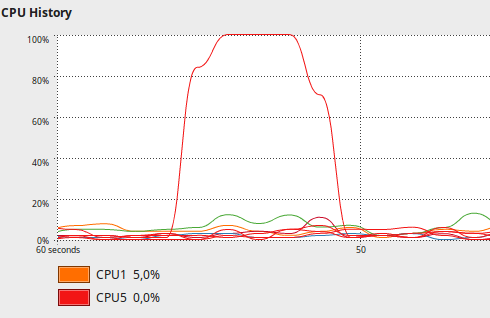
\includegraphics[width=\textwidth]{33-1.png}
        \caption{Jeden wątek}
        \label{fig:33-1}
    \end{subfigure}
    \begin{subfigure}[b]{0.4\textwidth}
        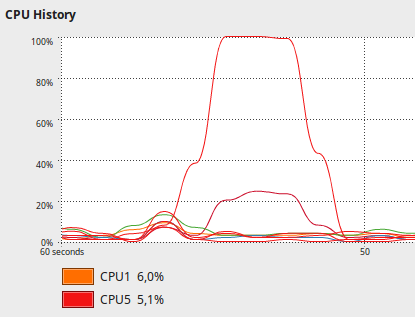
\includegraphics[width=\textwidth]{33-2.png}
        \caption{Dwa wątki}
        \label{fig:33-2}
    \end{subfigure}
    
    \begin{subfigure}[b]{0.4\textwidth}
        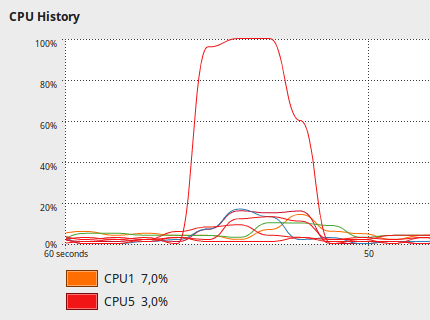
\includegraphics[width=\textwidth]{33-4.png}
        \caption{Cztery wątki}
        \label{fig:33-4}
    \end{subfigure} 
    \begin{subfigure}[b]{0.4\textwidth}
            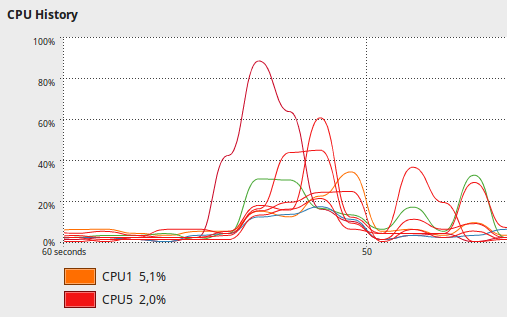
\includegraphics[width=\textwidth]{33-8.png}
            \caption{Osiem wątków}
            \label{fig:33-8}
    \end{subfigure}
    \caption{Fragmenty schematu ilustrującego zużycie rdzeni procesora przy użyciu (\ref{fig:33-1}) 1 wątku, (\ref{fig:33-2}) 2 wątków, (\ref{fig:33-4}) 4 wątków, (\ref{fig:33-8}) 8 wątków przy 500 miastach i wielkości populacji równej 100 (czwarte 4 wiersze tabeli)}\label{fig:33}. 
\end{figure}

\pagebreak
\section{Wnioski}
W celu zbadania najbardziej pracochłonnych części programu dokonano profilowania aplikacji przy użyciu programu \textit{callgrid}. Operacją, która trwa najdłużej jest krzyżowanie osobników. Dyrektywy \textit{OpenMP} w celu zrównoleglenia pętli zostały dodane w następujących miejscach:
\begin{itemize}
\item[--] operacja krzyżowania,
\item[--] operacja mutacji,
\item[--] obliczanie funkcji przystosowania dla osobników populacji,
\item[--] obliczanie prawdopodobieństwa osobnika do mechanizmu selekcji ruletkowej,
\item[--] konstruktor populacji - następuje w tym miejscu inicjalne tworzenie listy osobników na podstawie mapy miast na początku działania algorytmu.
\end{itemize}

Zrównoleglenie algorytmu za pomozą dyrektyw OpenMP powoduje około trzykrotne zmniejszenie czasu wykonania programu. Pliki wynikowe outSequence.txt i outParallel.txt przedstawiają Wyjście algorytmu w formie sekwencyjnej i zrównoleglonej Ze względu na ich długość poniżej zostały przedstawione niewielnie, lecz najważniejsze wycinki.

\begin{minted}{bash}
Parallel: whole_time = 40832015 microseconds
Sequential: whole_time = 16281865 microseconds
\end{minted}{bash}

Następują niewielkie wahania współczynnika przyspieszenia, ale generalnie utrzymuje się on na poziomie około 3 (trzyktotne przyspieszenie po użyciu dyrektyw OpenMP)
\subsection{Wnioski z przeprowadzonych testów}
Większa ilość testów przeprowadzonych na algorytmie z różnymi parametrami znajduje się w sekcji \ref{sec:wt}. Wnioski wysnute na jej podstawie można przedstawić następująco. 
\begin{itemize}
\item Zgodnie z oczekiwaniami wraz ze wzrostem ilości wątków czas wykonania programu ulega skróceniu.
\item Kiedy liczba miast jest znacznie większa od wielkości populacji wyniki zrównoleglenia dają zadowalające rezultaty, za to kiedy wielkość populacji jest porównywalna z liczbą miast w danym osobniku zrównoleglenie nie odnosi wielkiego skutku
\item Powodem takich wyników jest fakt że aplikacja jest zrównoleglona na poziomie populacji(czyli osobniki w populacji są przetwarzane równocześnie, ale jednocześnie każdy osobnik jest krzyżowany sekwencyjnie przez jeden wątek). Sprawia to, że im dłuższy osobnik względem rodzaju populacji tym zrównoleglenie jest efektywniejsze. 
\item Wraz z powiększeniem wymiaru problemu przez zwiększenie liczby miast zrównoleglenie wykonania algorytmu powoduje lepsze rezultaty, ponieważ stosunek najbardziej pracochłonnych fragmentów programu, w których zastosowano dyrektywy OpenMP w celu zrównoleglenia, do reszty programu jest większy niż w przypadku małych problemów. 
\item Metoda koła ruletki powoduje,że wraz ze wzrostem liczby pokoleń algorytm ewoluuje coraz wolniej (dochodzi do powolnej stagnacji).
\end{itemize}


\end{document}
